\chapter{Inferring evolutionary parameters of colorectal cancer from DNA methylation arrays}\label{methchap}
\section{Introduction}
The model discussed in this report is the $1$D version of the agent-based model \texttt{demon} developed by Rob. All rates and are given relative to the birth rate which is assumed to be equal to $1$ (as per the Gillespie algorithm).
\section{Results}
I performed the preliminary sensitivity analysis on a small set of simulations, more as a sanity check than a robust test. However, the results are interesting as the model is more sensitive to some parameters than expected. The parameters, checked are ones controlling selective advantage, driver mutation rates, fCpG flipping probabilities, and gland fission rates.
\subsection{A note on the fully neutral model}
As discussed in previous meetings, the fully neutral model does not behave as expected. Instead, its outputs look like they are just oscillations around the initial fCpG array. This, I think, is due to the lack any preference for one lineage over any other within a gland, leading to a decoherence of the arrays after a long period of turnover, but without any resolution in space/time. However, even with selective advantage for driver mutations within glands, the glands themselves undergo fission in space neutrally as there is no competition for space in the model. The limitations of this assumption need to be discussed, but it seems reasonable for now.

\subsection{Selective advantage}
The selective advantage, accounted for in the model as
\begin{equation}
    \lambda' = \lambda\left(1 + s\left(\frac{\lambda}{\lambda_{max}}\right)\epsilon\right),
\end{equation}
where $\lambda$ is the birth rate before mutation, $\lambda'$ is the birth rate after mutation, $\lambda_{max}$ is the maximal allowed birth rate, and $\epsilon$ is a unit exponentially distributed value. The values of $s$ tested were $0.1$, $0.2$, and $0.3$ with the other parameters kept at values given in table \ref{tab:parameters}.
\begin{figure}[h]
    \centering
    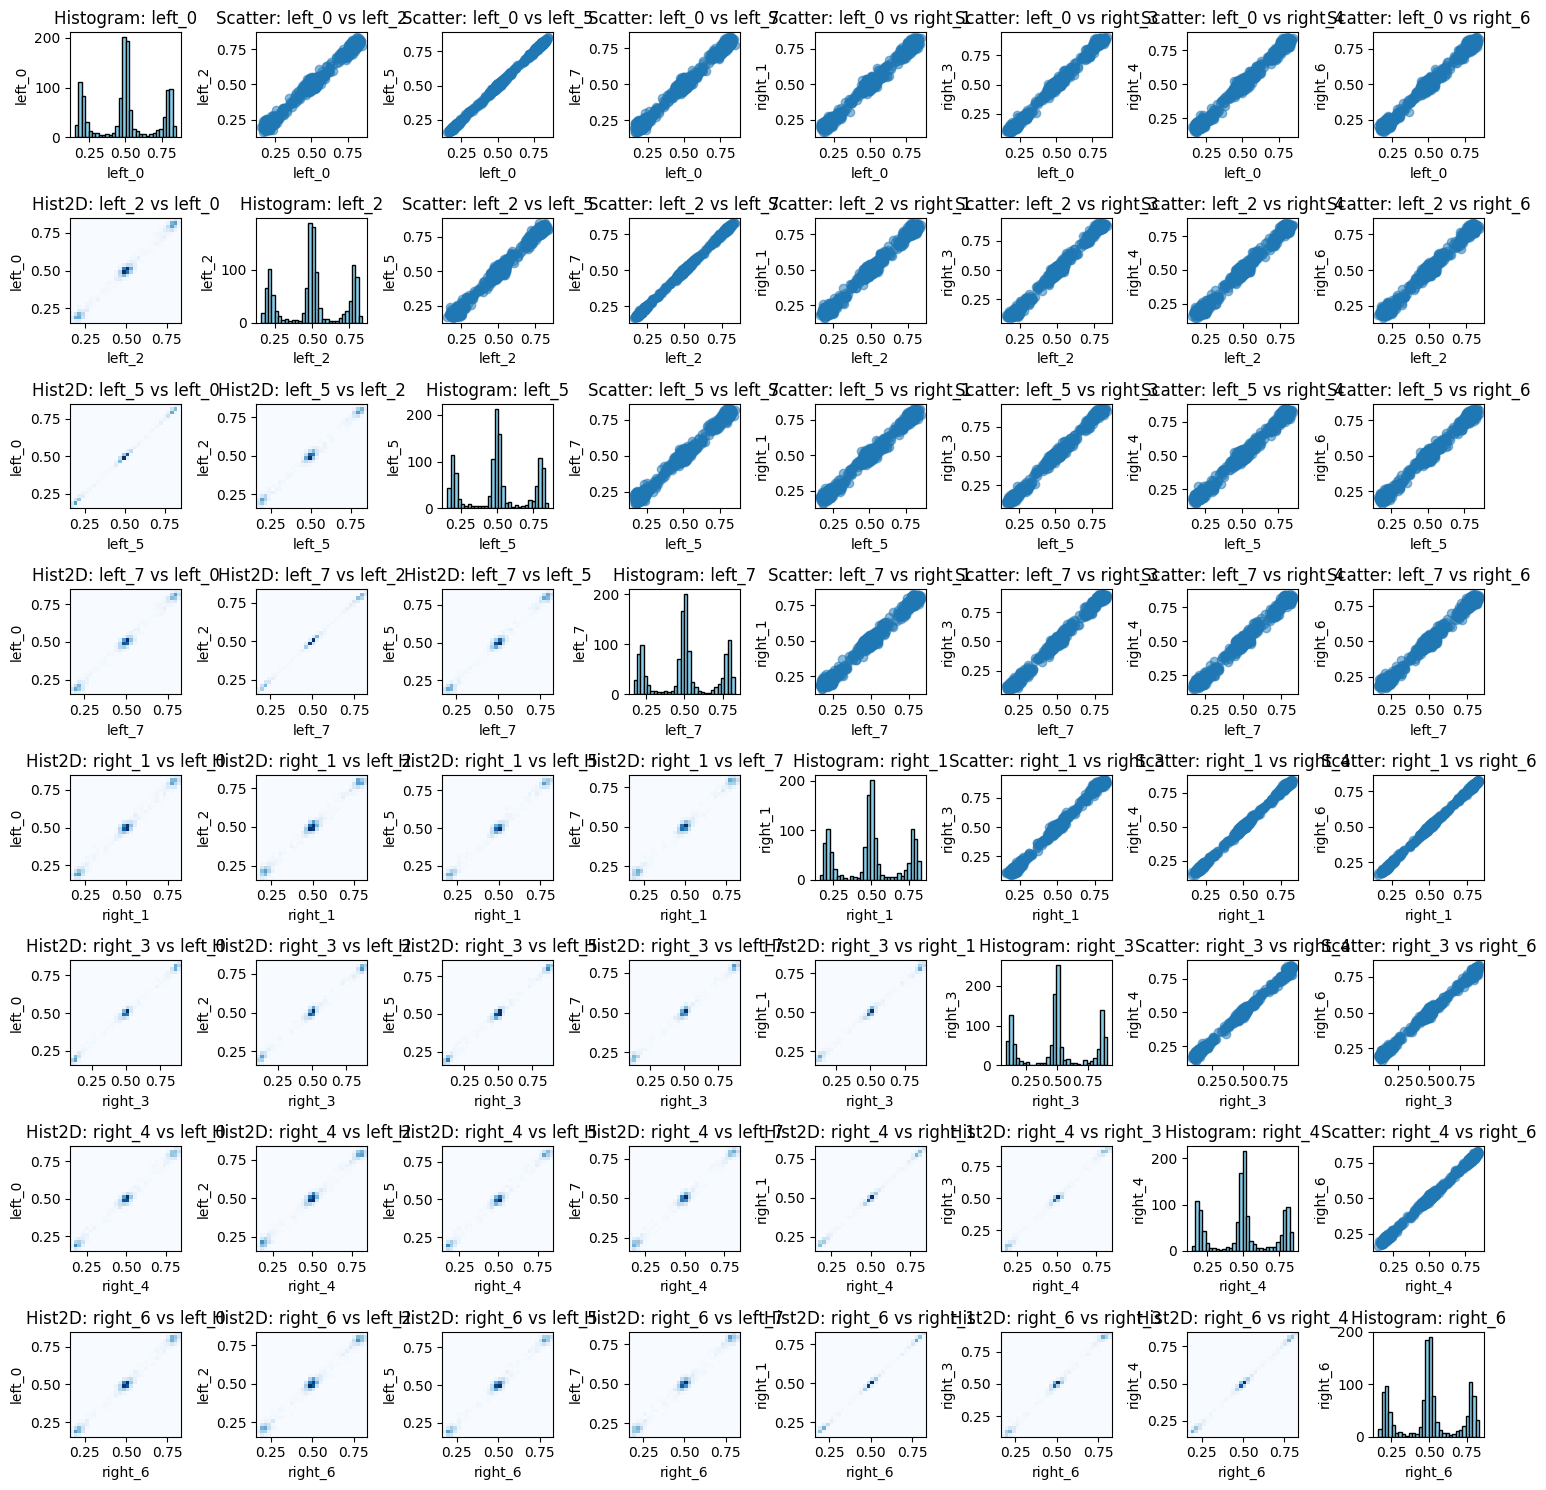
\includegraphics[width=\textwidth]{Chapter_methylation/figures/sensitivity_selective_advantage1.png}
    \caption{correlation scatter plots, gland histograms and correlation heatmaps for $s=0.1$.}
    \label{fig:sensitivity_selective_advantage1}
\end{figure}
\begin{figure}[h]
    \centering
    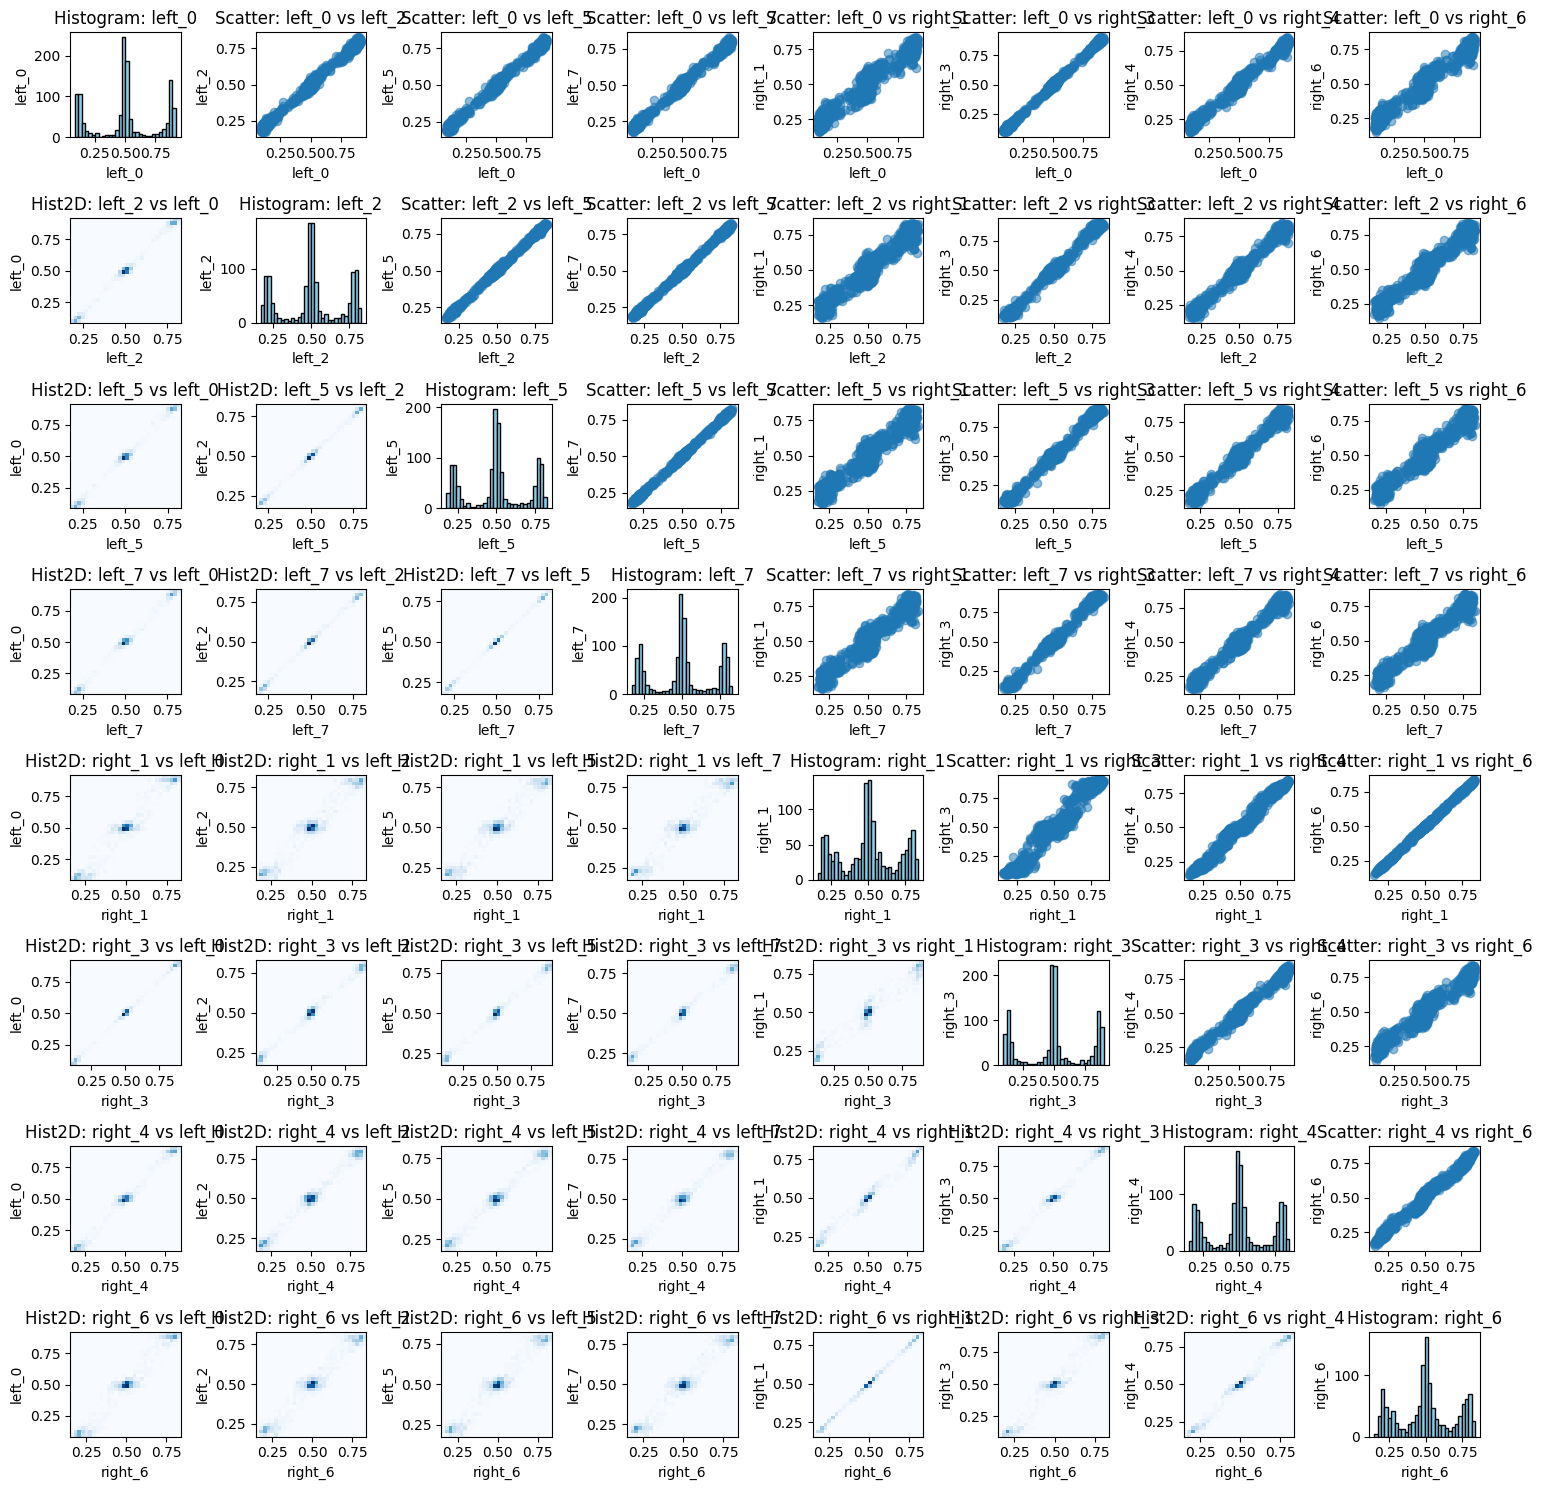
\includegraphics[width=\textwidth]{Chapter_methylation/figures/sensitivity_selective_advantage2.png}
    \caption{correlation scatter plots, gland histograms and correlation heatmaps for $s=0.2$.}
    \label{fig:sensitivity_selective_advantage2}
\end{figure}
\begin{figure}[h]
    \centering
    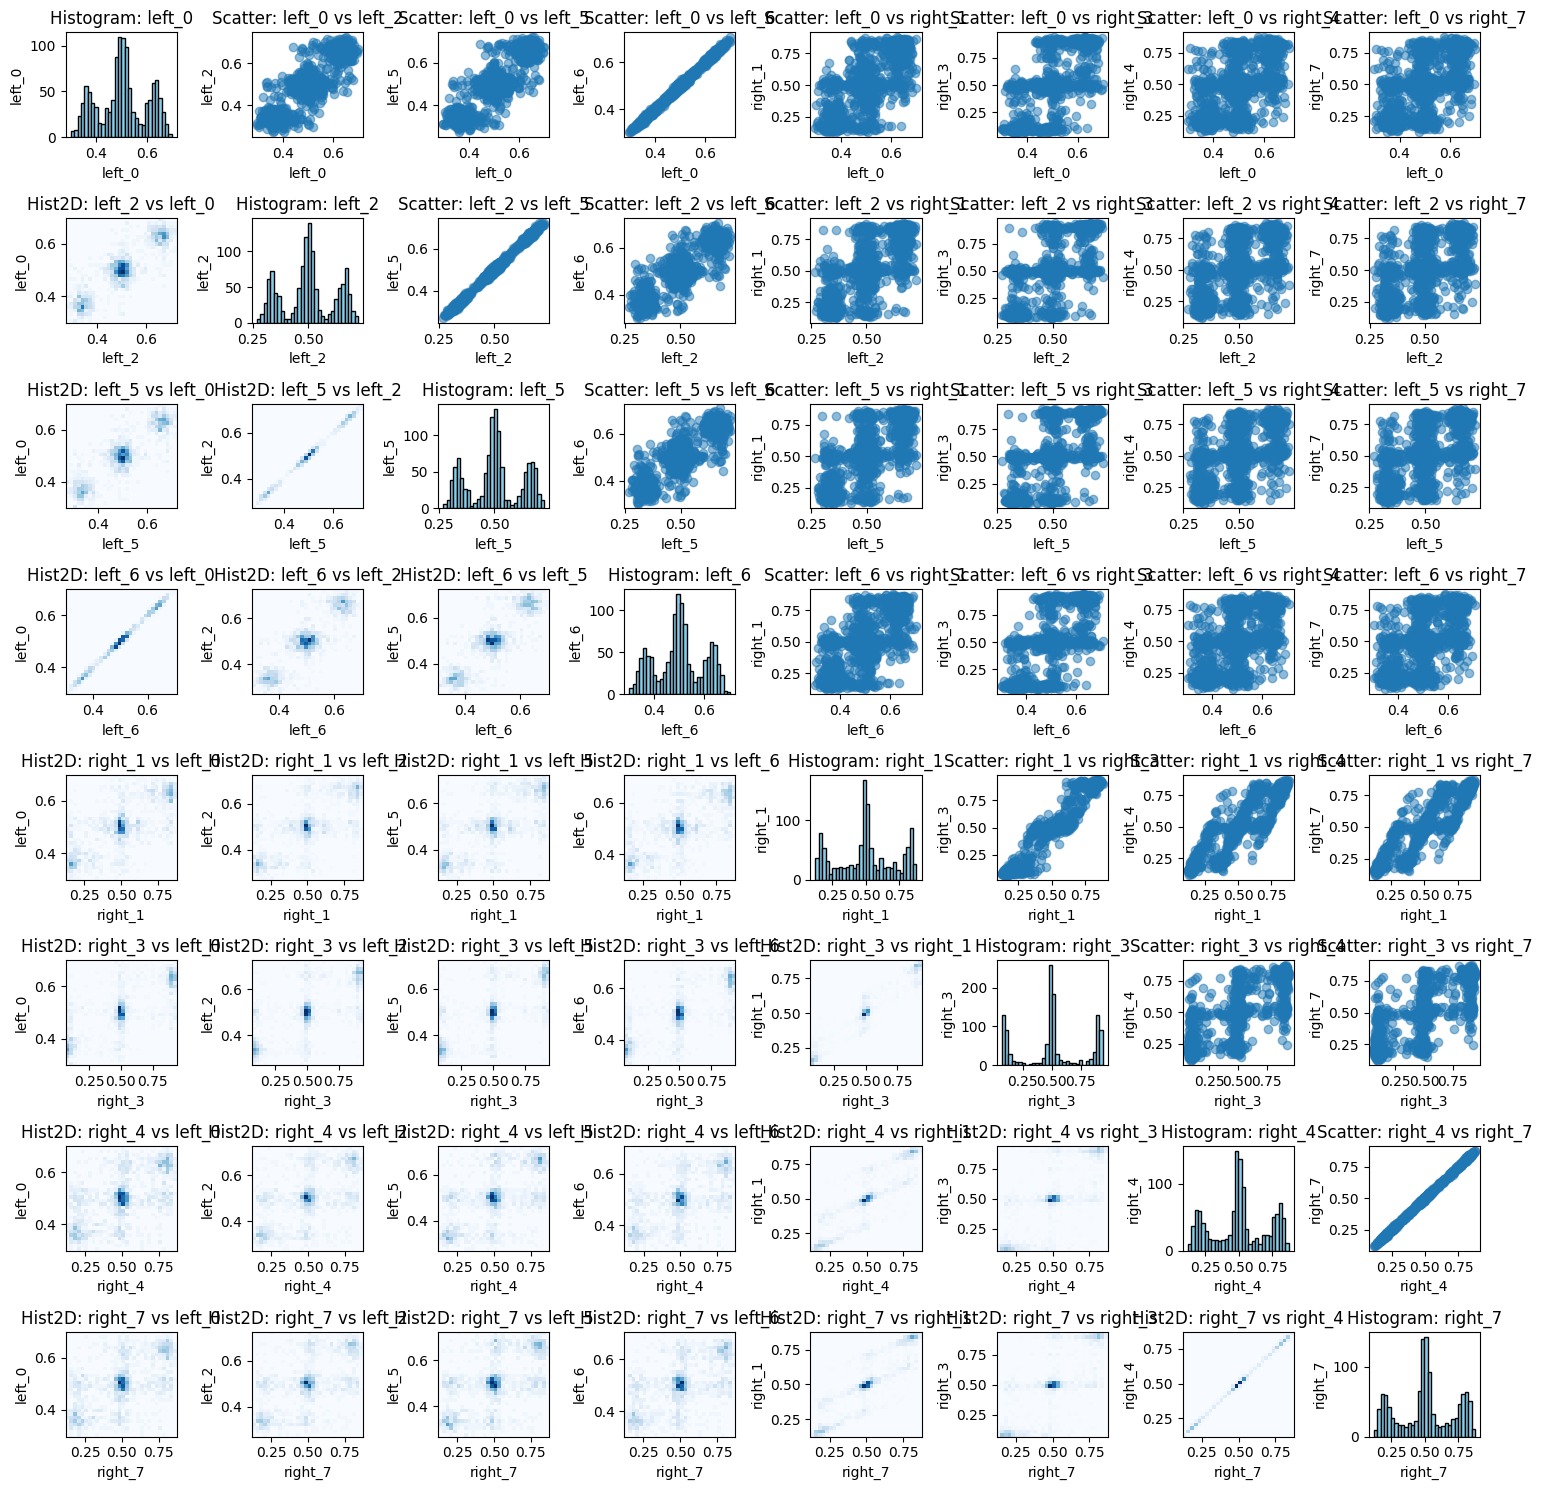
\includegraphics[width=\textwidth]{Chapter_methylation/figures/sensitivity_selective_advantage3.png}
    \caption{correlation scatter plots, gland histograms and correlation heatmaps for $s=0.3$.}
    \label{fig:sensitivity_selective_advantage3}
\end{figure}
In addition to the fully neutral model not recapitulating the patterns observed in data, it seems the weak selection regimes have a similarly hard time establishing lineages which would lead to decoupling between sides of the tumour.
\clearpage
\subsection{Driver mutation rates}
The driver mutation rates were tested at $10^{-6}$ and $10^{-4}$ with the other parameters kept at values given in table \ref{tab:parameters}, and the case for the mutation rate equal to $10^{-5}$ covered in figure \ref{fig:sensitivity_selective_advantage3}.
\begin{figure}[h]
    \centering
    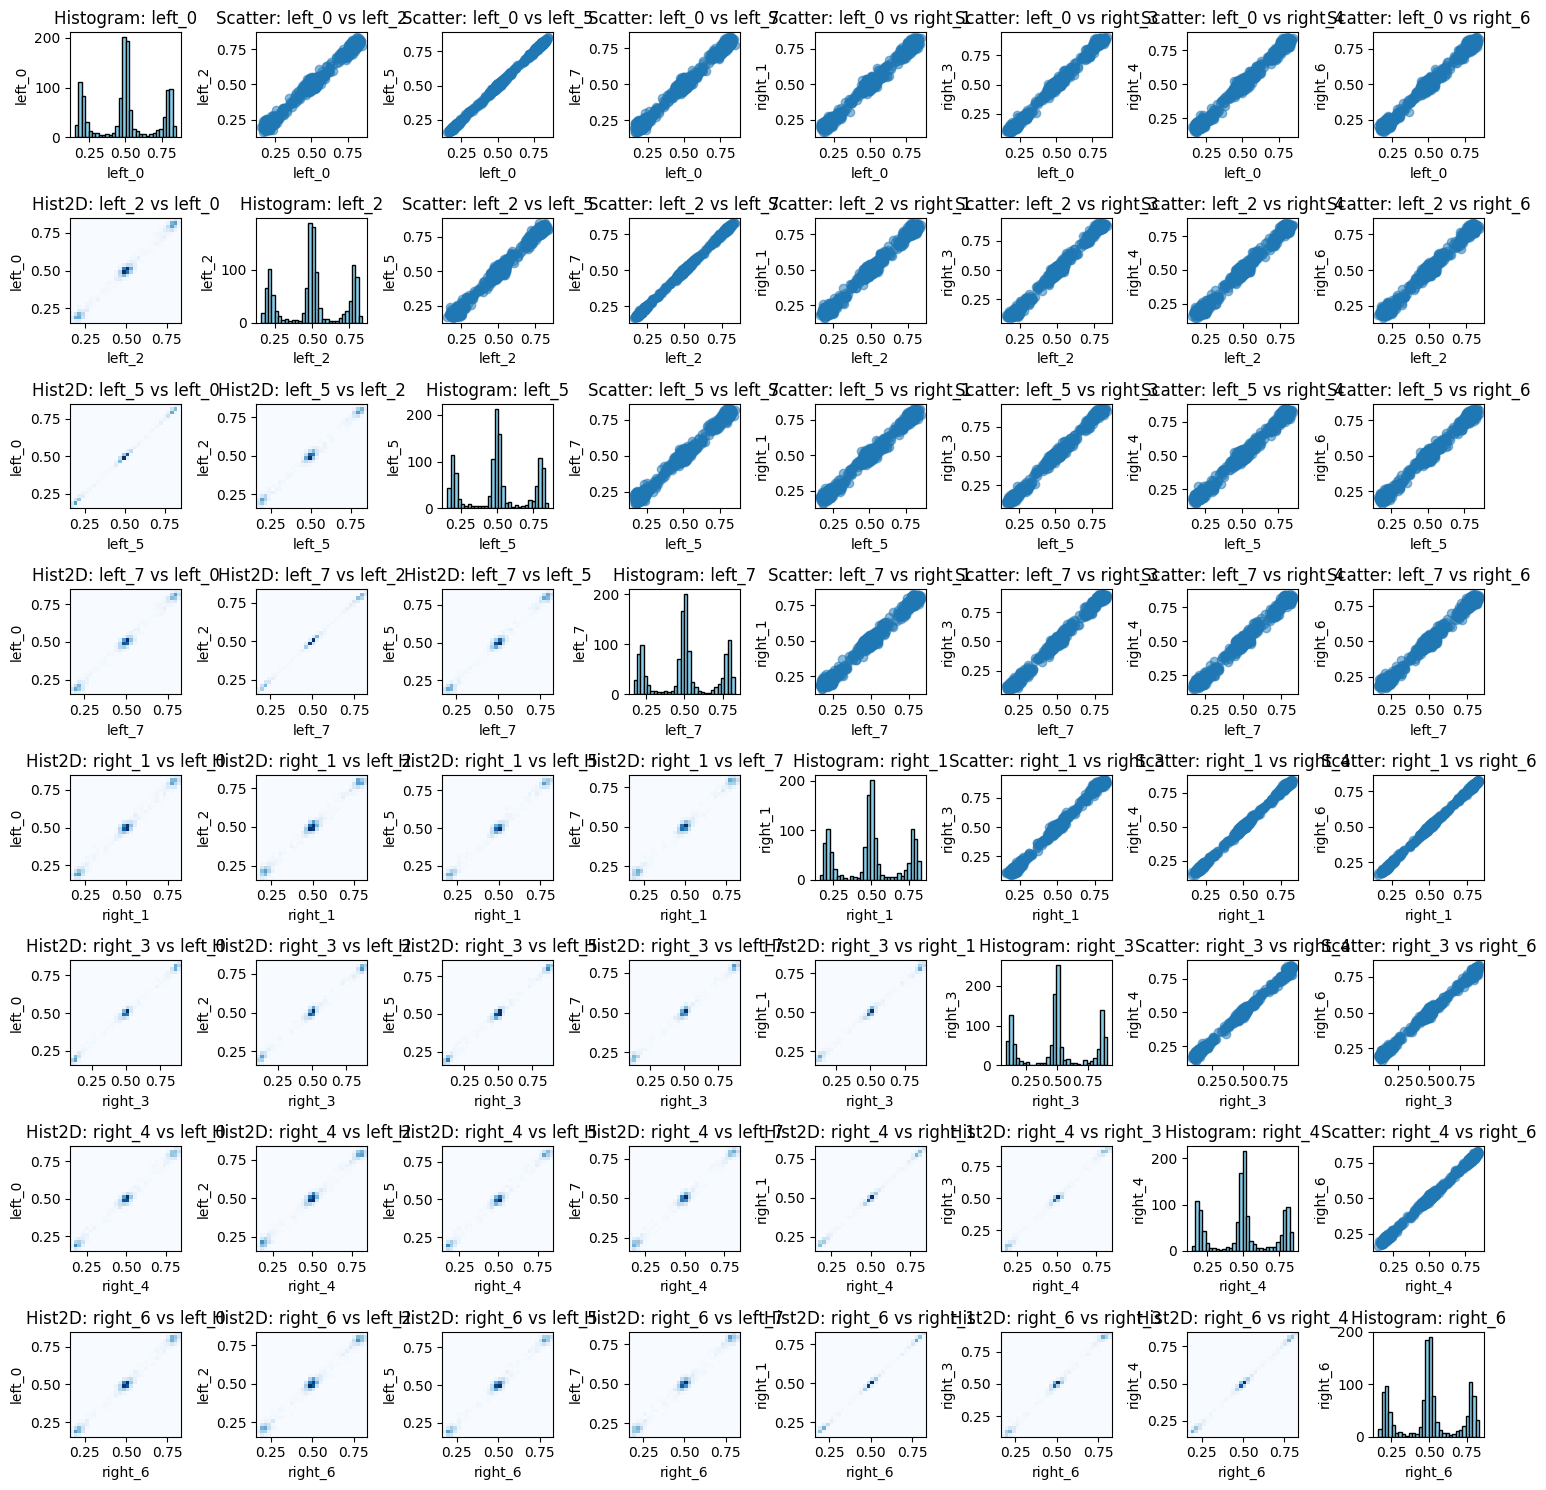
\includegraphics[width=\textwidth]{Chapter_methylation/figures/sensitivity_driver1.png}
    \caption{correlation scatter plots, gland histograms and correlation heatmaps for driver mutation rate $10^{-6}$.}
    \label{fig:sensitivity_driver1}
\end{figure}
\begin{figure}[h]
    \centering
    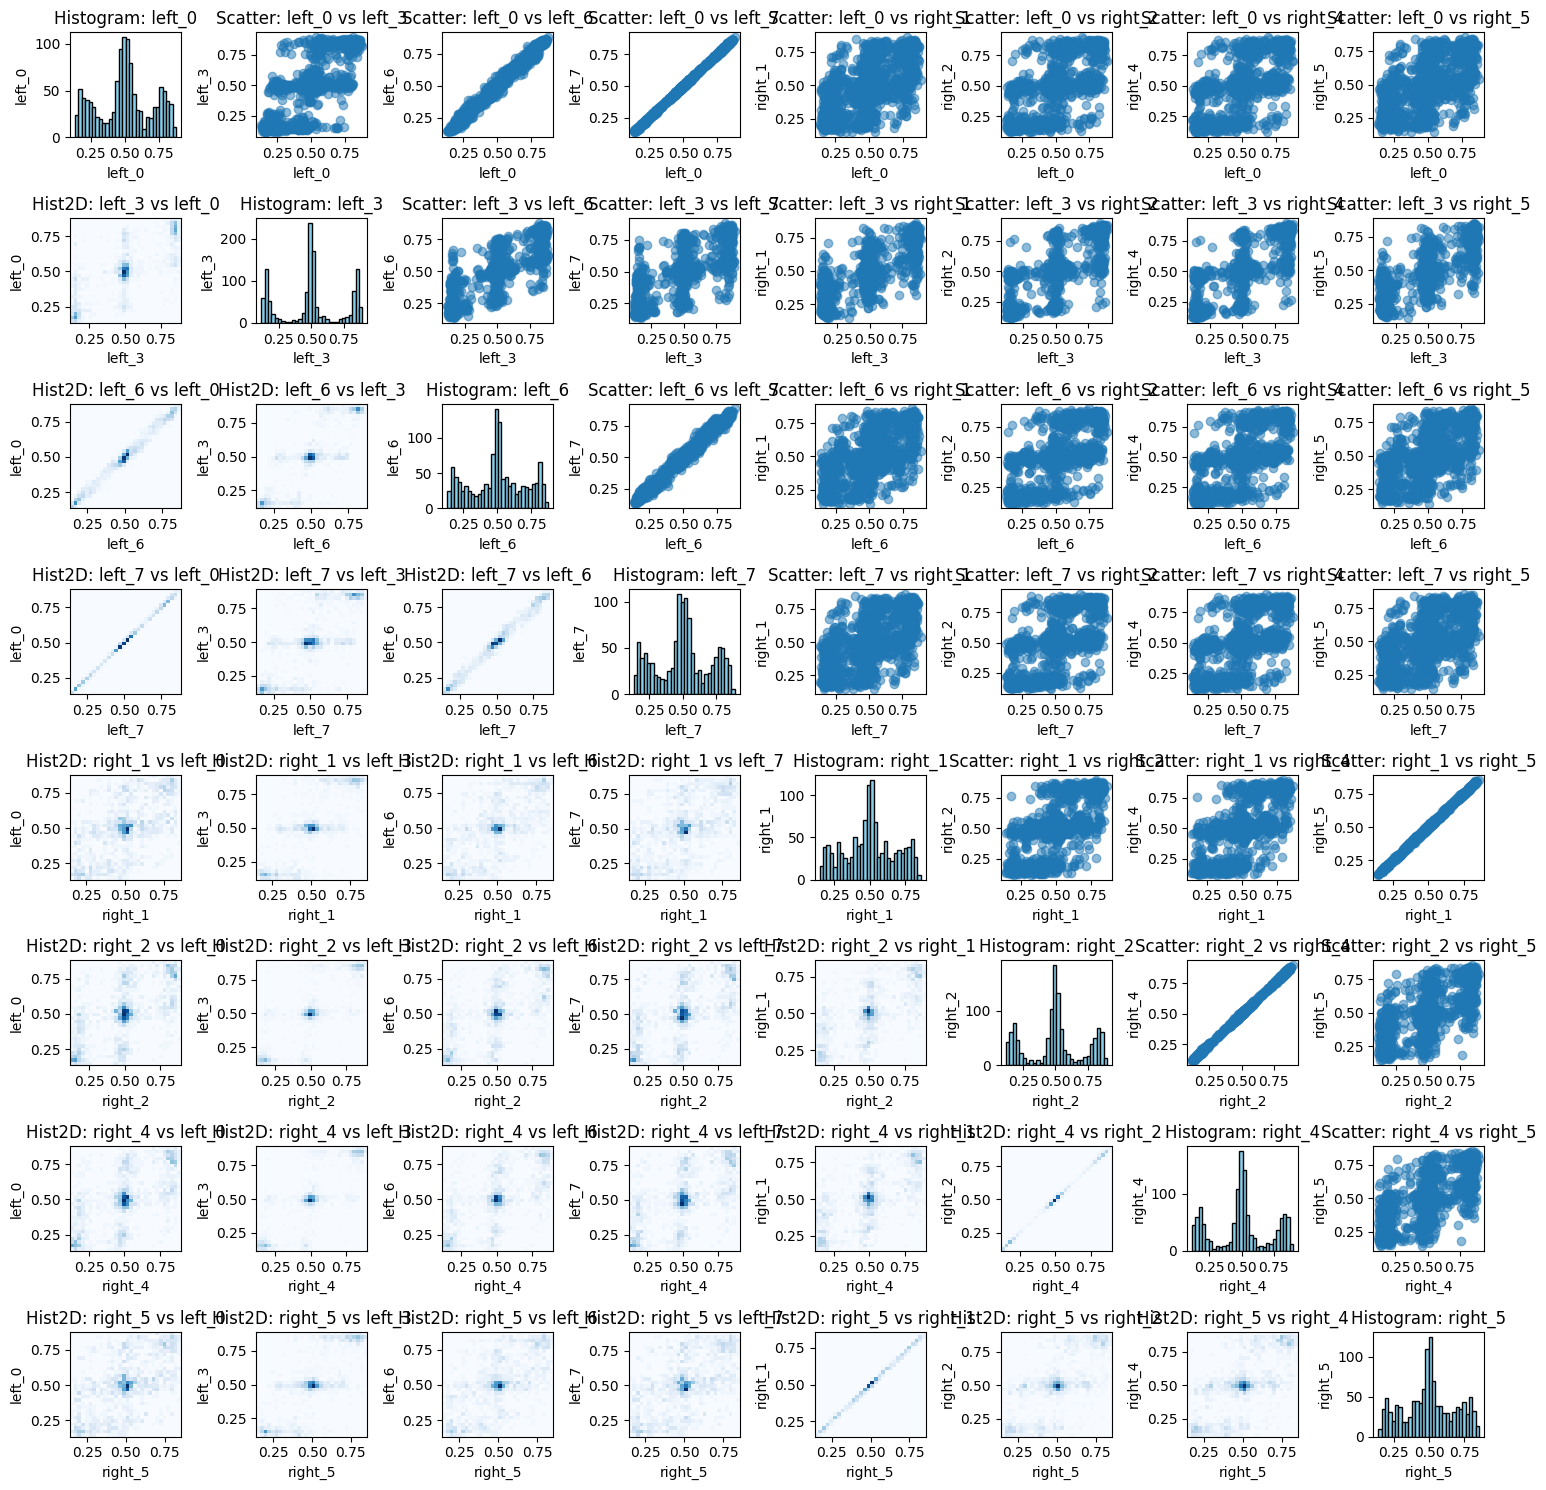
\includegraphics[width=\textwidth]{Chapter_methylation/figures/sensitivity_driver2.png}
    \caption{correlation scatter plots, gland histograms and correlation heatmaps for driver mutation rate $10^{-4}$.}
    \label{fig:sensitivity_driver2}
\end{figure}
\clearpage
\subsection{fCpG flipping probabilities}
The fCpG flipping probabilities were tested at $10^{-4}$, $10^{-3}$, and $10^{-2}$ with the other parameters as in table \ref{tab:parameters}. The case for $5\times10^{-3}$ is covered by figure \ref{fig:sensitivity_selective_advantage3}. \par
\begin{figure}[h]
    \centering
    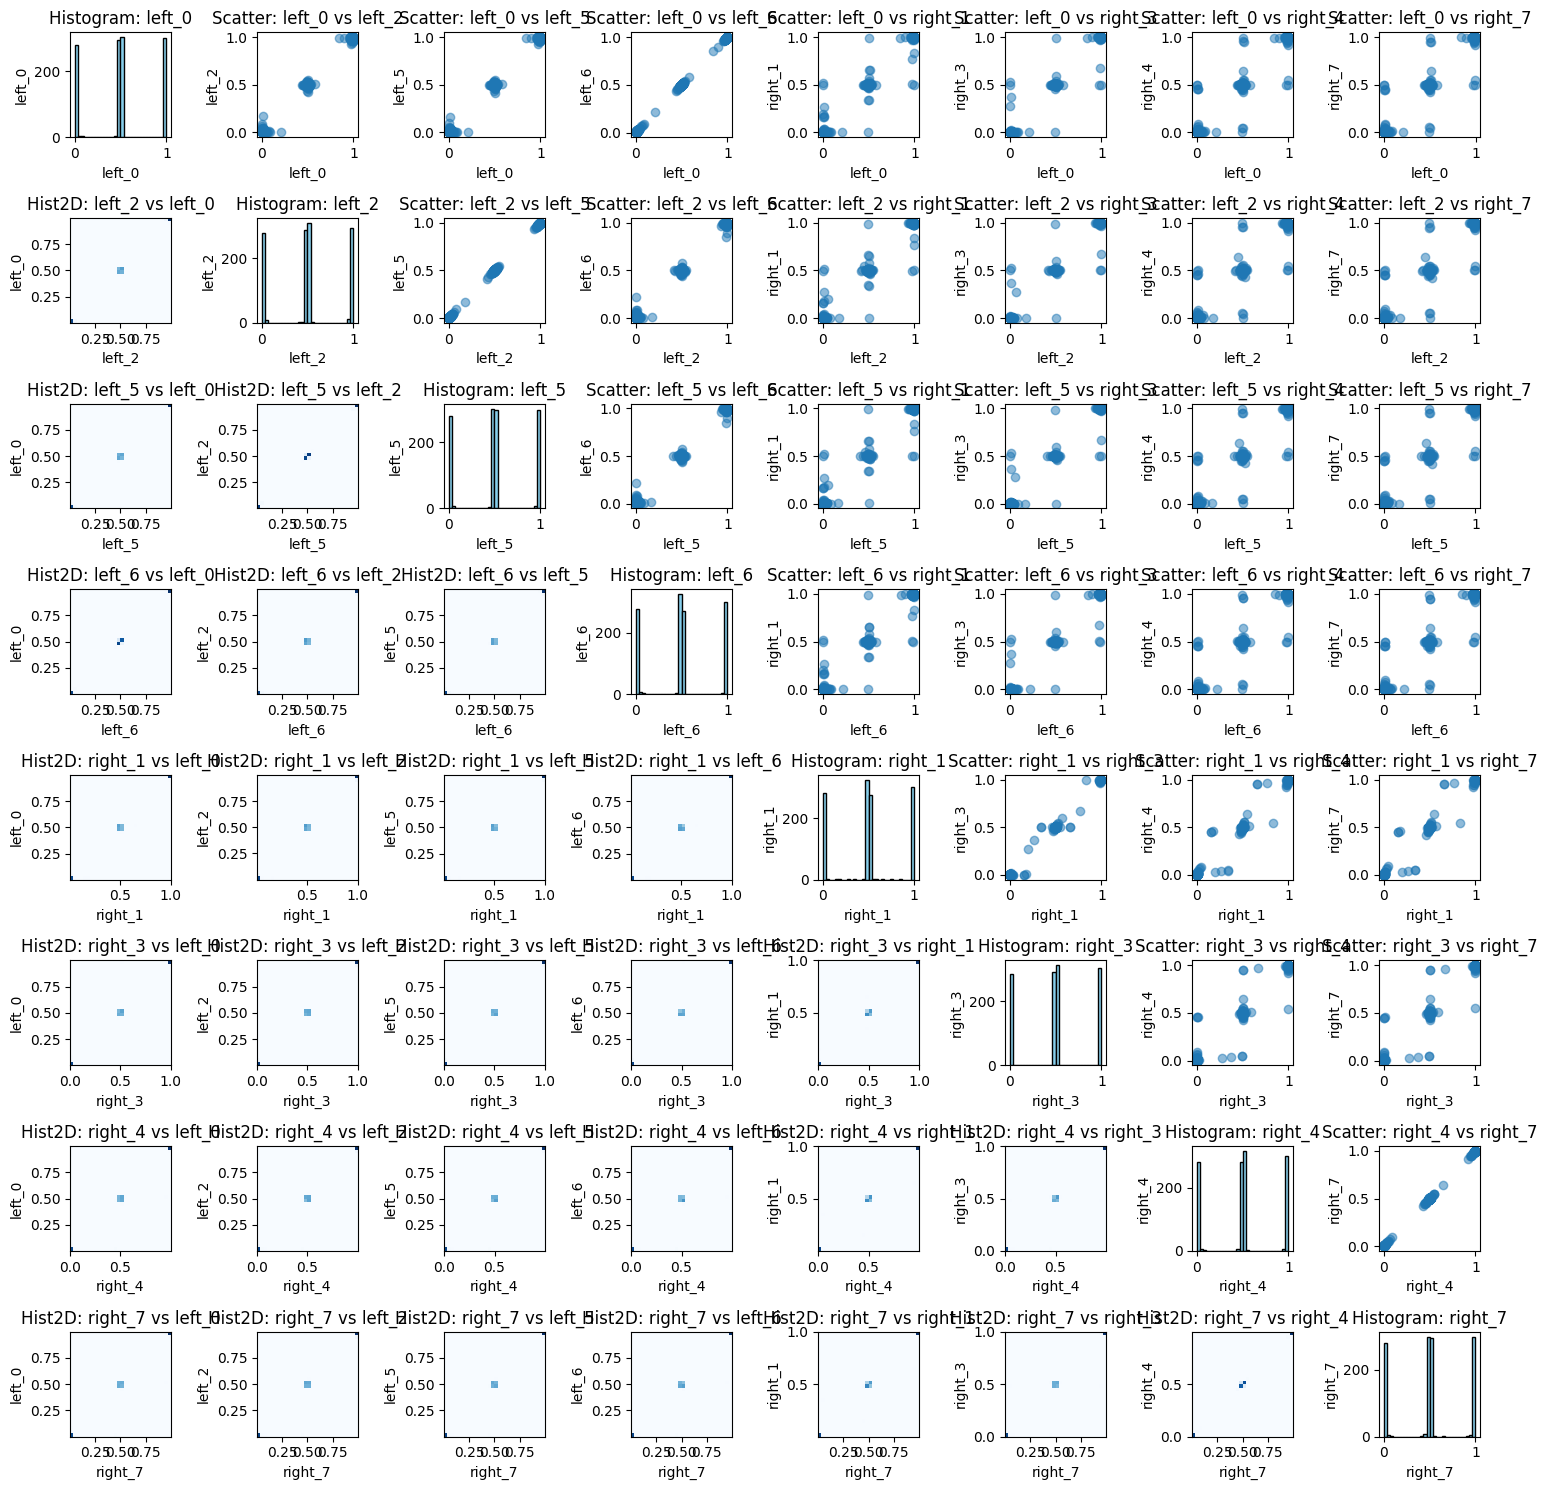
\includegraphics[width=\textwidth]{Chapter_methylation/figures/sensitivity_flipprob1.png}
    \caption{correlation scatter plots, gland histograms and correlation heatmaps for flip probabilities $10^{-4}$.}
    \label{fig:sensitivity_flipprob1}
\end{figure}
\begin{figure}[h]
    \centering
    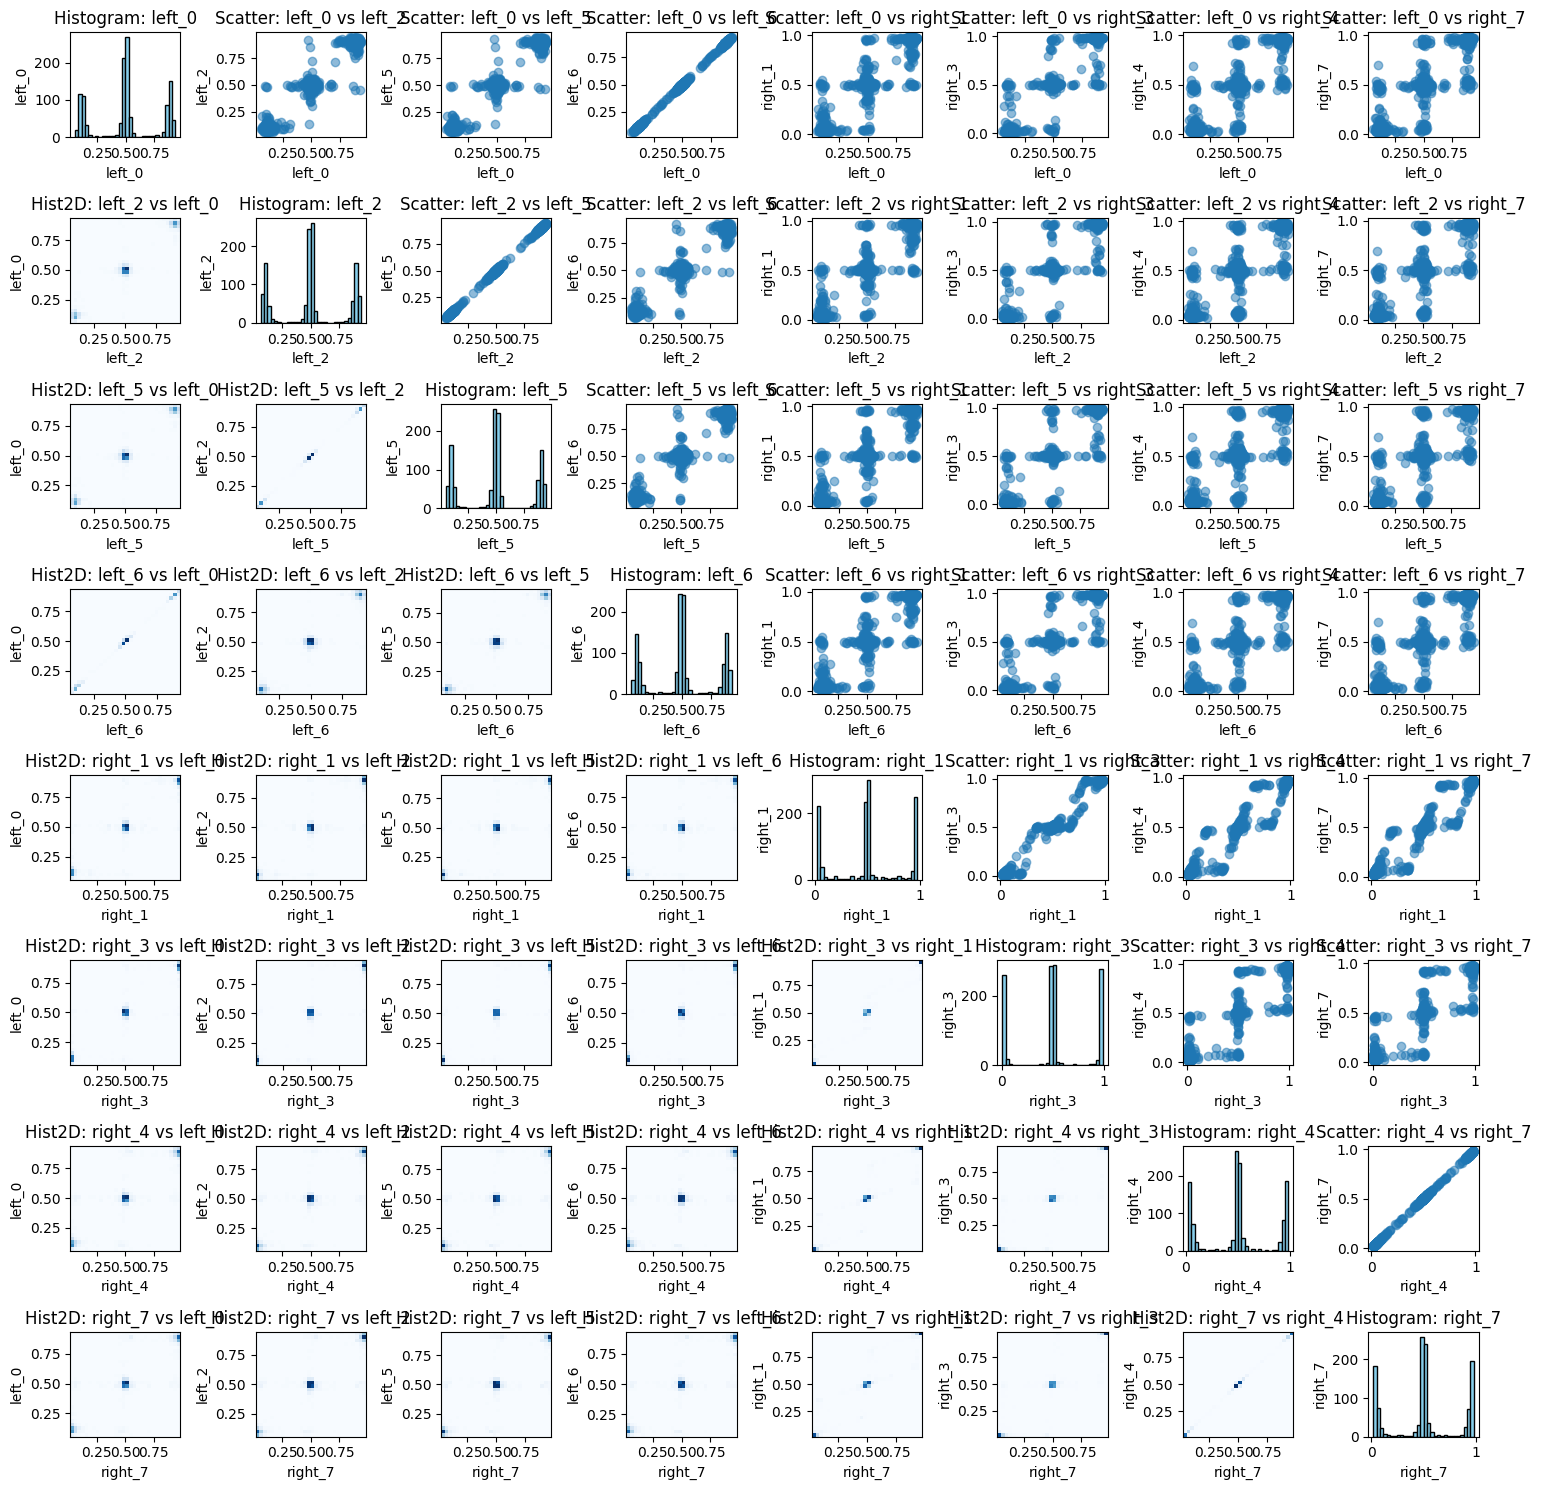
\includegraphics[width=\textwidth]{Chapter_methylation/figures/sensitivity_flipprob2.png}
    \caption{correlation scatter plots, gland histograms and correlation heatmaps for flip probabilities $10^{-3}$.}
    \label{fig:sensitivity_flipprob2}
\end{figure}
\clearpage
\begin{figure}[h]
    \centering
    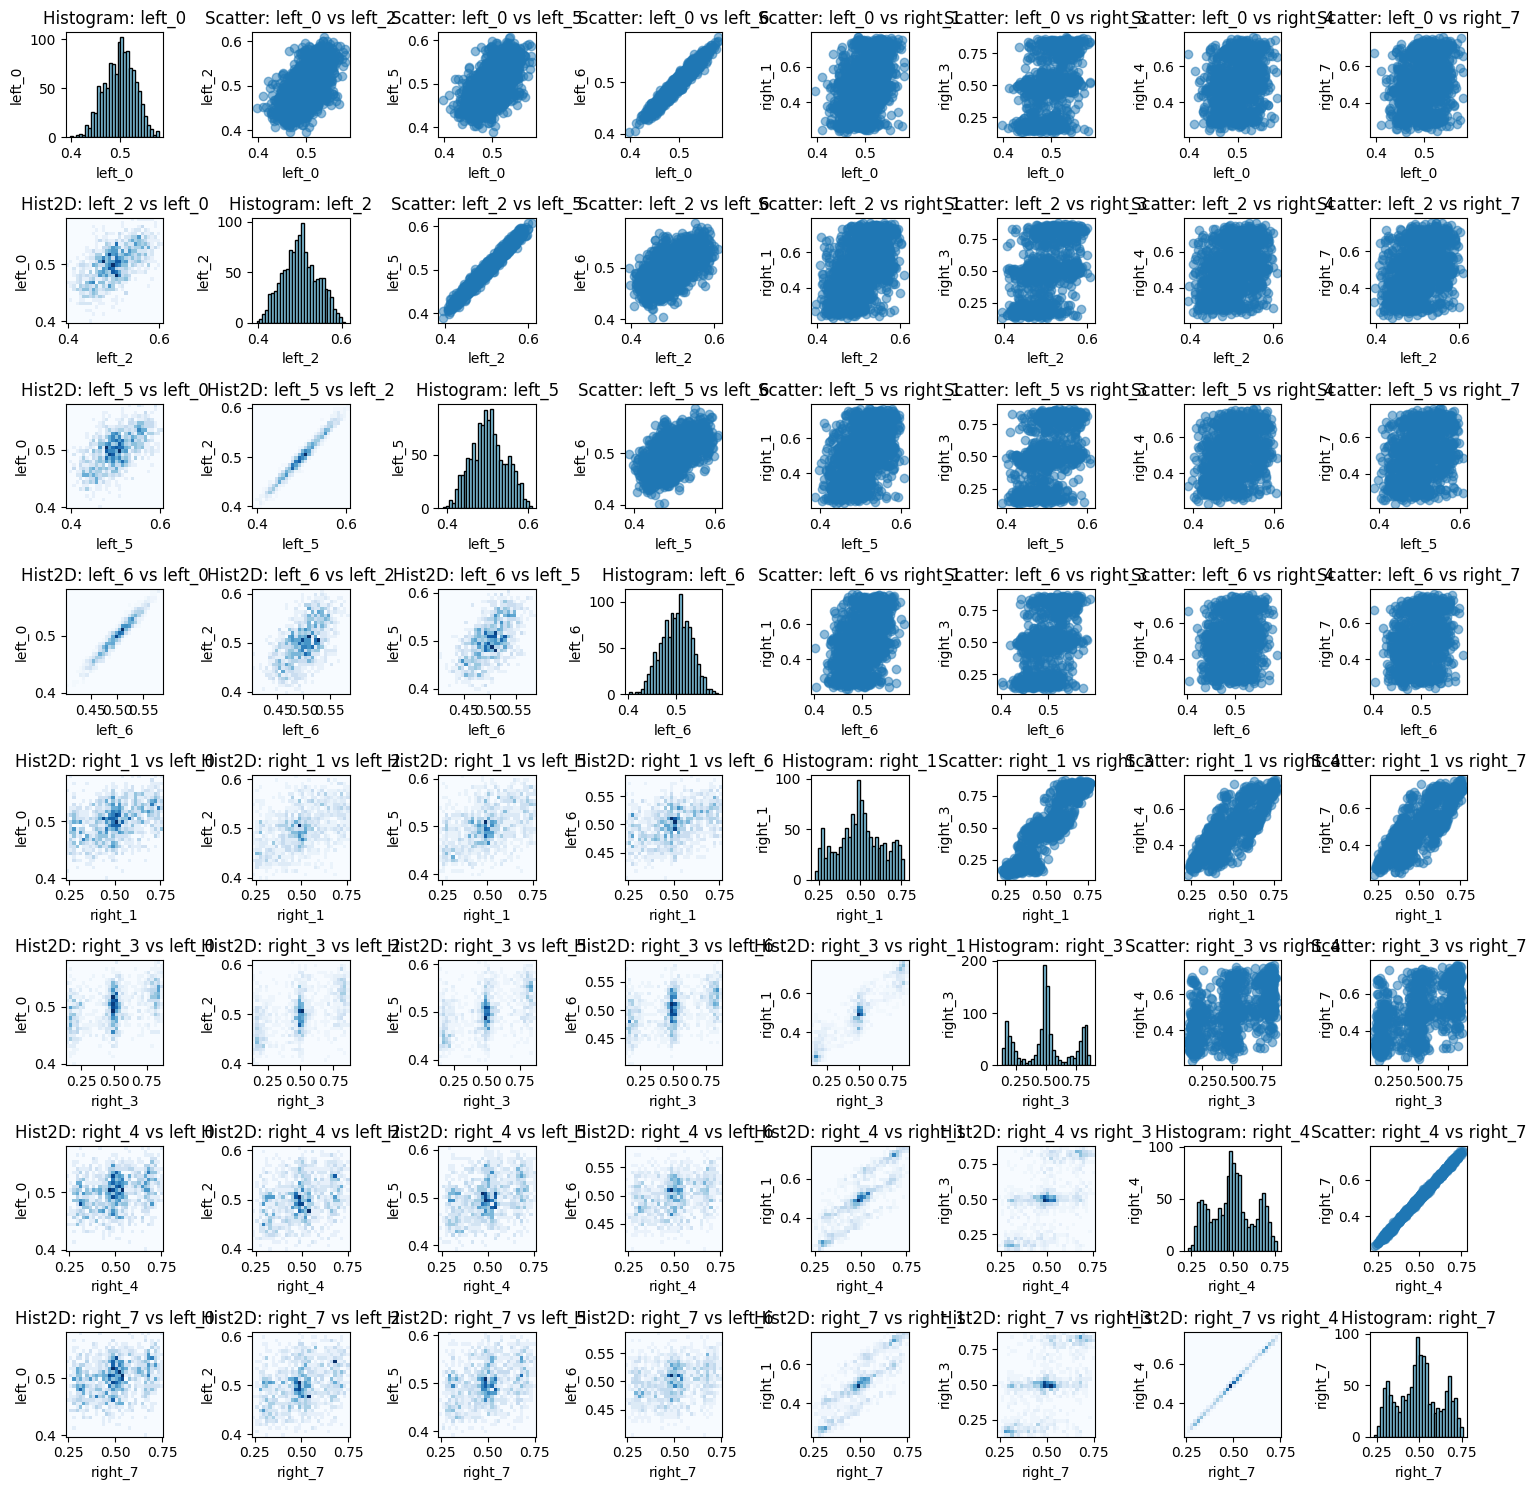
\includegraphics[width=\textwidth]{Chapter_methylation/figures/sensitivity_flipprob3.png}
    \caption{correlation scatter plots, gland histograms and correlation heatmaps for flip probabilities $10^{-2}$.}
    \label{fig:sensitivity_flipprob3}
\end{figure}
\clearpage
As expected, the higher probabilities lead to quicker decoupling, even between glands which are on the same side of the tumour. On the other hand, lower probabilities show very little change between the initial and final arrays.

\subsection{Gland fission rates}
The gland fission rates tested were $0.008$, $0.08$, and $0.8$. The other parameters were kept as in table \ref{tab:parameters}. The case of $0.008$ did not produce any fissions and is not included below, and the case of $0.08$ had a total of $4$ fissions which resulted in $5$ glands at the end of the simulation. The case for fission rates equal to $0.4$ was covered in figure \ref{fig:sensitivity_selective_advantage3}.
\begin{figure}[h]
    \centering
    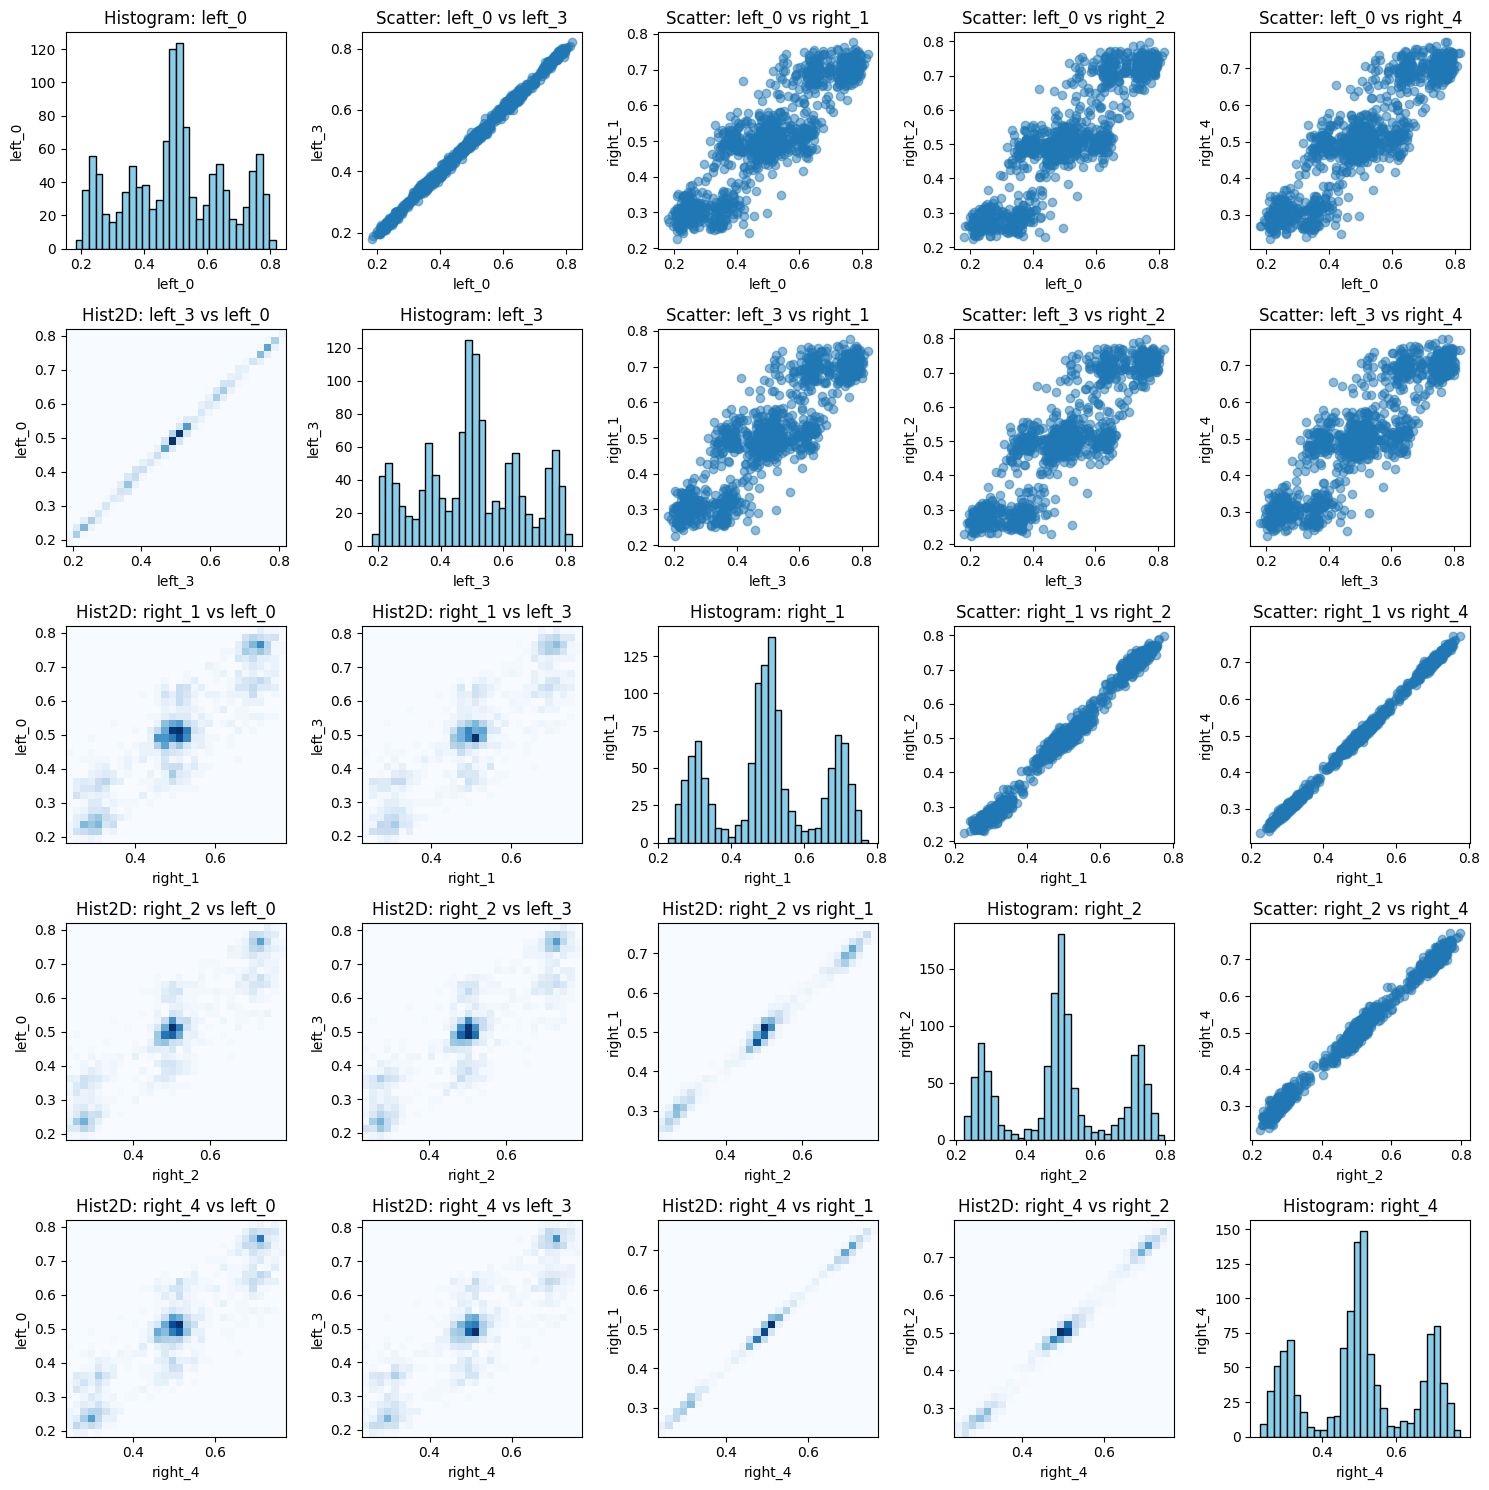
\includegraphics[width=\textwidth]{Chapter_methylation/figures/sensitivity_migrate1.png}
    \caption{correlation scatter plots, gland histograms and correlation heatmaps for fission rates $0.008$.}
    \label{fig:sensitivity_migrates1}
\end{figure}
\begin{figure}[h]
    \centering
    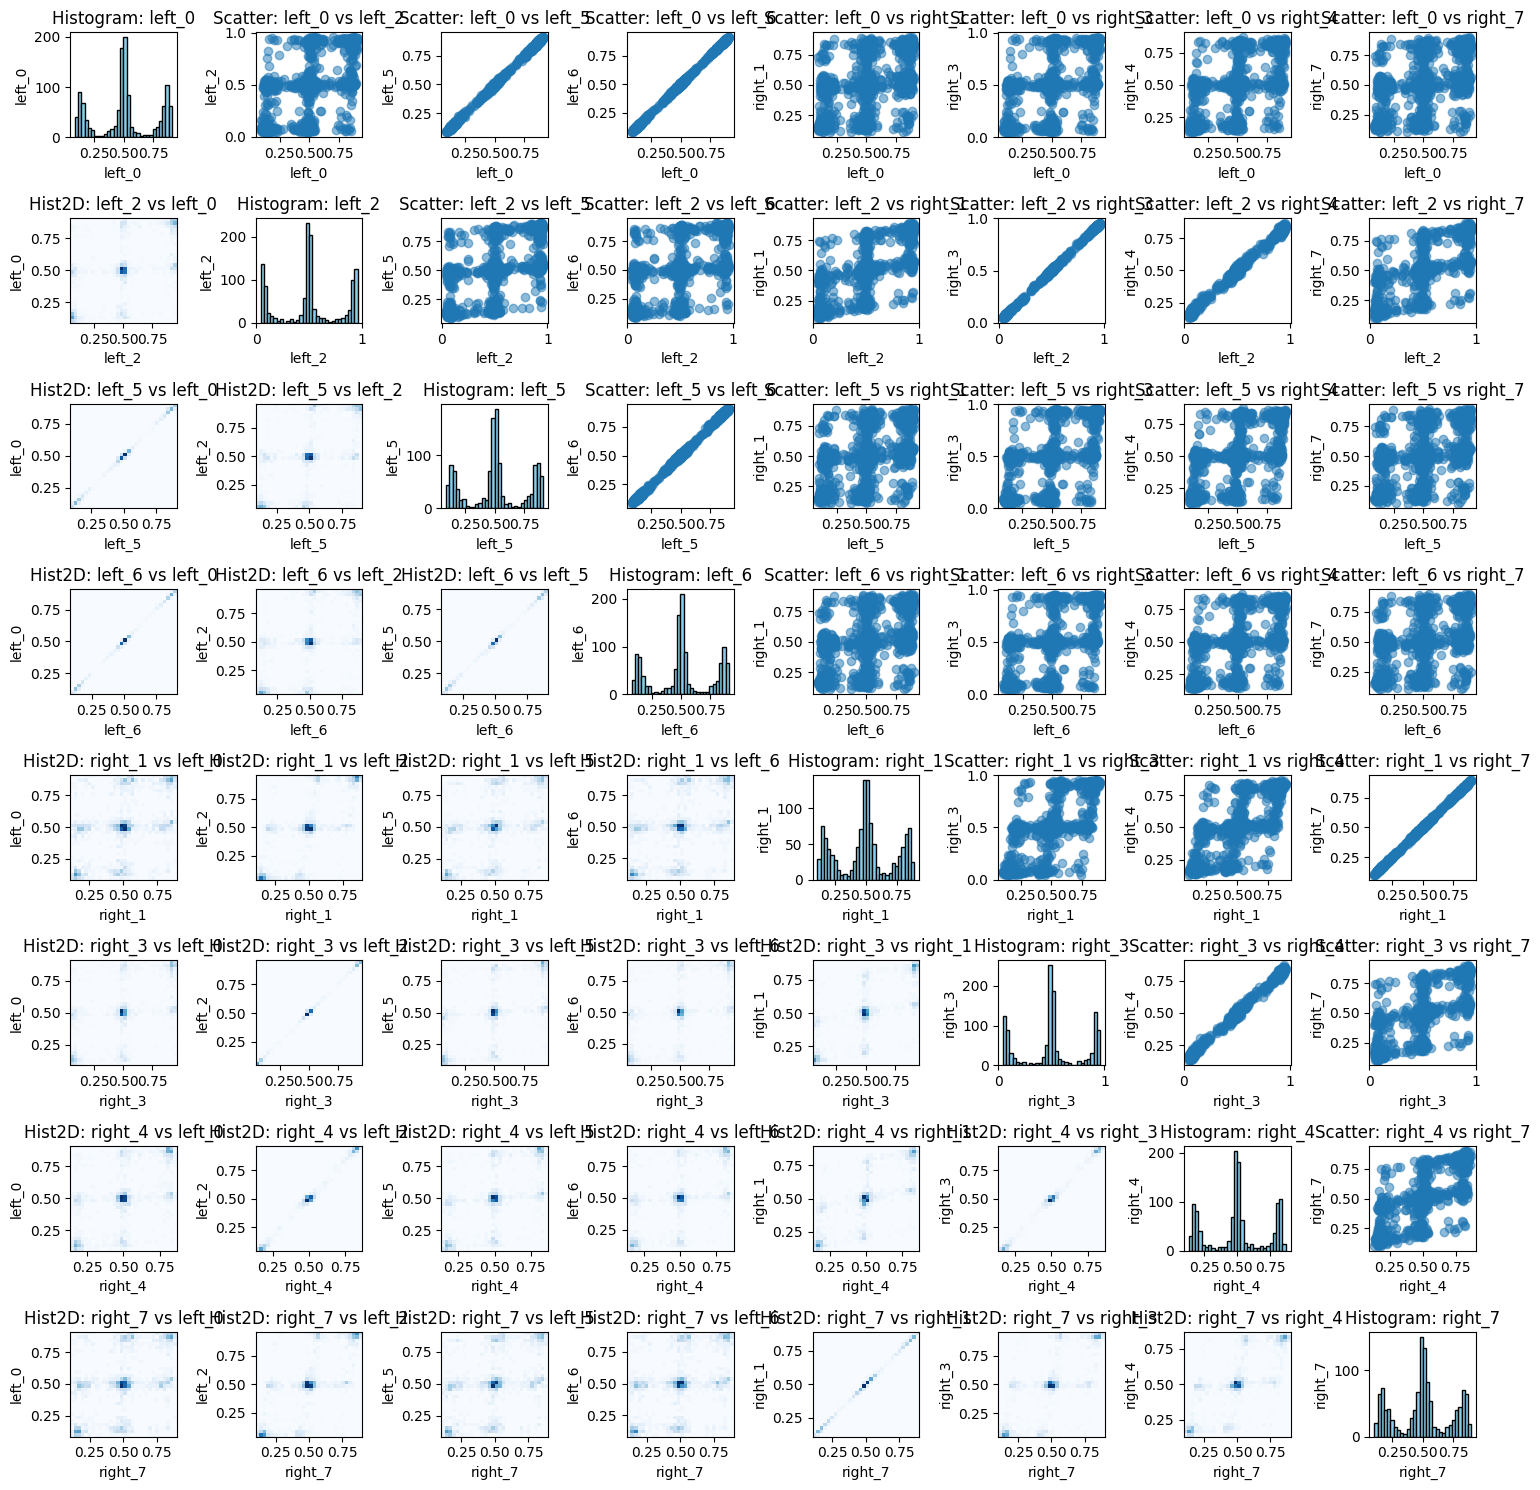
\includegraphics[width=\textwidth]{Chapter_methylation/figures/sensitivity_migrate2.png}
    \caption{correlation scatter plots, gland histograms and correlation heatmaps for fission rates $0.08$.}
    \label{fig:sensitivity_migrate2}
\end{figure}
\clearpage
Nominally, faster fission rates should lead to less time spent in turnover before fission, and therefore less time for the fCpG sites to decouple. However, I set these simulations up with that in mind so that the glands spend around $40\%$ of the simulated time in turnover.

\section{Parameters}
The loose default parameter settings used in the simulations are given in Table \ref{tab:parameters}.

\begin{table}[ht]
\centering
\begin{tabular}{|l|l|}
\hline
Parameter & Value \\
\hline
    Driver mutation rate & $10^{-5}$   \\
    Methylation probability per fCpG site per cell division & $5\times10^{-3}$ \\
    Demethylation probability per fCpG site per cell division & $5\times10^{-3}$ \\
    Gland fission rate & $0.4$  \\
    Cells per gland & 8192 \\
    fCpG loci per cell & 1200 \\
    Selective advantage & $0.3$ \\
\hline
\end{tabular}
\caption{Default parameter values.}\label{tab:parameters}
\end{table}
The values are educated guesses based on the two fCpG papers. The simulations were run for $50$ Gillespie generations, which equated to tumours between 10 and 50 glands across. The tumours were allowed about $40\%$ of the growth time in turnover. The simulations were run on my laptop, I am currently scaling the framework up for deployment on City's computing cluster.\par

\section{Distance functions}
The basic distance functions I have started from are inspired by the Metropolitan distance. The distance between site $A$ in gland $2$ and site $A$ in gland $2$ is calculated as the classic Metropolitan distance with a modification that the values of $A_1$ and $A_2$ are put in bins based on their proximity to the values of $0$, $0.5$, and $1$. The main difference between distance functions I've experimented with is adjusting the value added to the distance based on the difference between sites in different glands.
\begin{figure}[h]
    \centering
    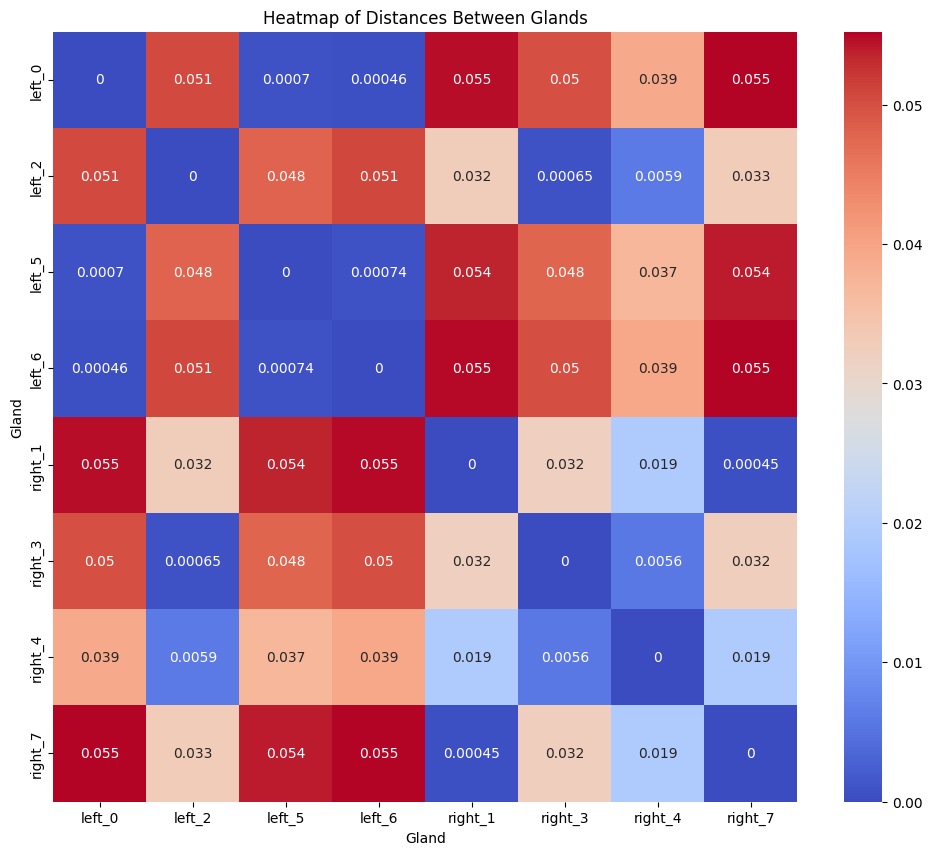
\includegraphics[width=\textwidth]{Chapter_methylation/figures/sensitivity_migrate2_distances.png}
    \caption{Distances between glands from figure \ref{fig:sensitivity_migrate2}.}
    \label{fig:distance_functions}
\end{figure}
\begin{figure}[h]
    \centering
    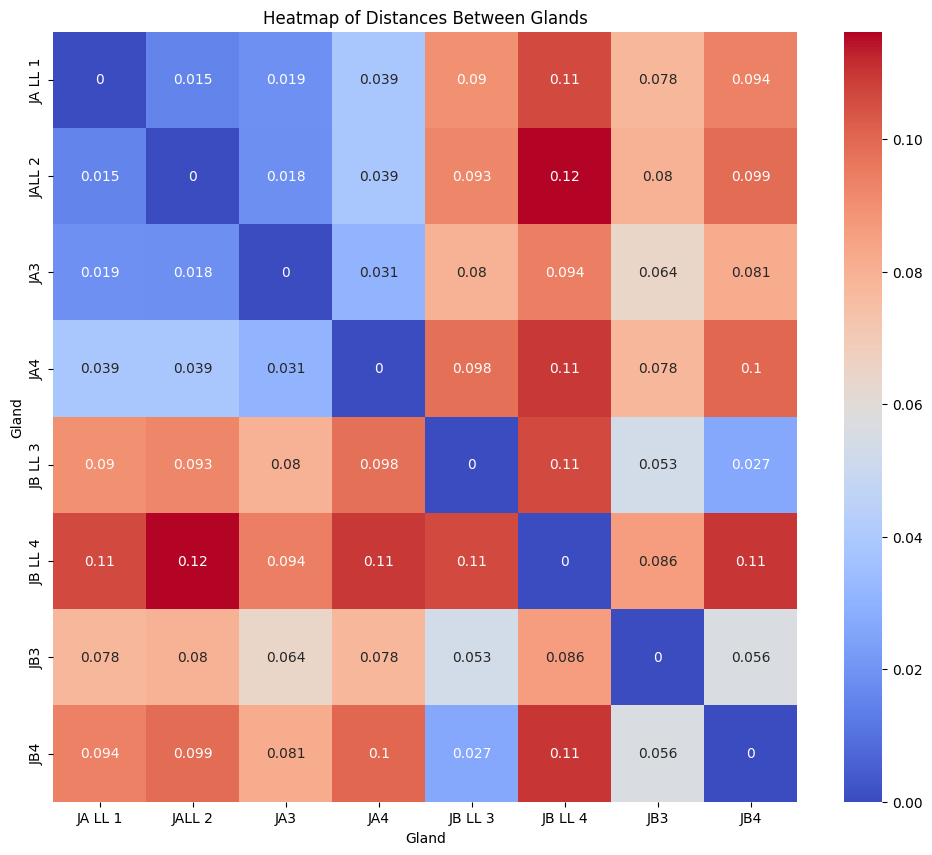
\includegraphics[width=\textwidth]{Chapter_methylation/figures/data_example_distances.png}
    \caption{Distances between glands from data set J.}
    \label{fig:data_distances}
\end{figure}
\begin{figure}[h]
    \centering
    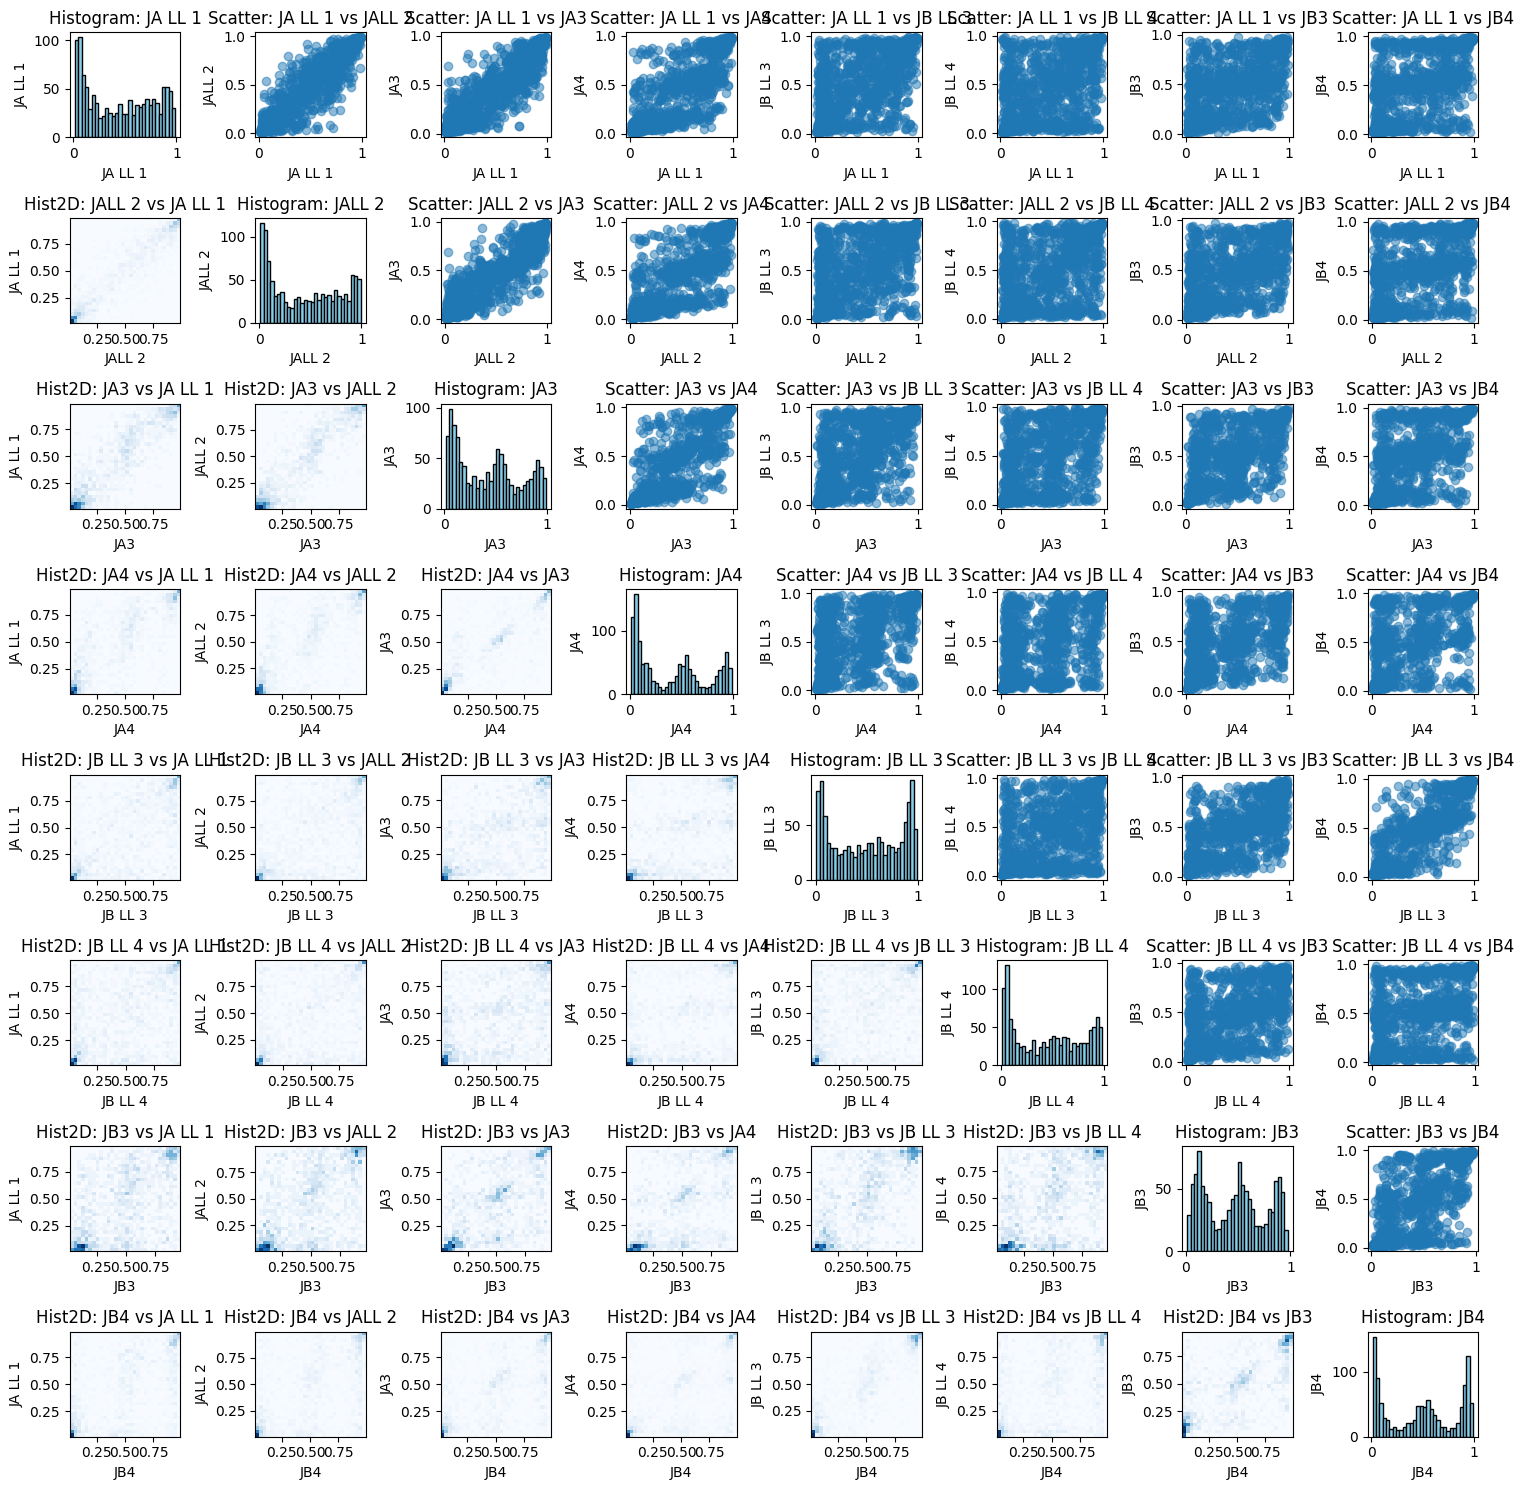
\includegraphics[width=\textwidth]{Chapter_methylation/figures/data_example_corrs.png}
    \caption{Data set J whose distances are shown in \ref{fig:data_distances}.}
    \label{fig:data_example_corrs}
\end{figure}
\clearpage
\section{Next steps/work in progress}
Currently working on the following:
\begin{itemize}
    \item Grid search over the above parameter space to check whether there are clusters which correspond to different tumour growth regimes.
    \item Refining the distance functions to better capture the differences between the arrays.
\end{itemize}
Next on the list:
\begin{itemize}
    \item Inferring parameters from synthetic data based on the above two steps.
    \item Inference of parameters or qualitative properties of real data sets - depends on the results of the above.
\end{itemize}

\subsection{Hypotheses}
\begin{itemize}
    \item \texttt{methdemon} recapitulates FMC patterns in colorectal cancer. \textbf{Test:} Extensive sensitivity analysis of \texttt{methdemon} and comparison to a different model (A/B model test with a simpler model, rule out trivial and, ideally, non-trivial models).
    \item \texttt{methdemon} reproduces evolutionary dynamics of colorectal cancer (effectively neutral). \textbf{Test:} Inferring parameters from simulations --- under consideration are fission rate, mutation rate, time under turnover.
    \item stem cell hypothesis - assume expansion process for each lineage and draw all cells within glands from distribution (multinomial or whatever). polyclonal origin - easy to test (fully neutral).
    \item Spatial resolution is needed to recover evolutionary dynamics of colorectal cancer. \textbf{Test:} Compare \texttt{methdemon} to EVOFLUx (average over the data for each cancer to run the latter).
    \item FMC patterns imply evolutionary bottlenecks between distant glands in colorectal cancer. \textbf{Test:} Develop distance metric, run EVOFLUx on individual glands (or a variation of EVOFLUx). NOTE: ask Darryl if he can be more specific on which bottlenecks he means. Need specific things that can be implemented in the model.
\end{itemize}

